\documentclass{minimal}
\usepackage{graphicx,color}
\usepackage[papersize={576.00bp,432.00bp},text={576.00bp,432.00bp}]{geometry}
\begin{document}
\centering
% Title: glps_renderer figure
% Creator: GL2PS 1.3.8, (C) 1999-2012 C. Geuzaine
% For: Octave
% CreationDate: Tue Mar 15 17:45:57 2016
\setlength{\unitlength}{1pt}
\begin{picture}(0,0)
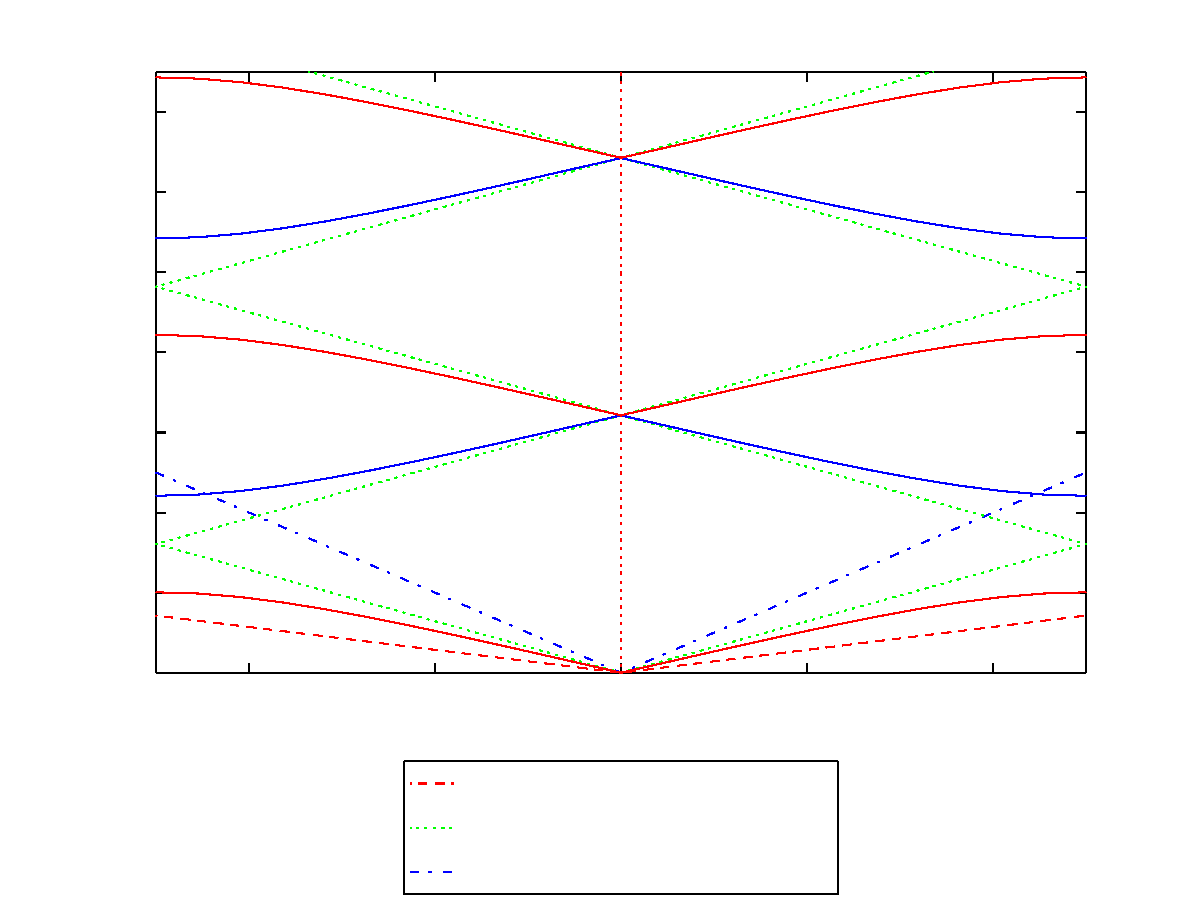
\includegraphics{lightcone_comparison-inc}
\end{picture}%
\begin{picture}(576,432)(0,0)
\fontsize{10}{0}
\selectfont\put(119.52,104.086){\makebox(0,0)[t]{\textcolor[rgb]{0,0,0}{{-0.4}}}}
\fontsize{10}{0}
\selectfont\put(208.8,104.086){\makebox(0,0)[t]{\textcolor[rgb]{0,0,0}{{-0.2}}}}
\fontsize{10}{0}
\selectfont\put(298.08,104.086){\makebox(0,0)[t]{\textcolor[rgb]{0,0,0}{{0}}}}
\fontsize{10}{0}
\selectfont\put(387.36,104.086){\makebox(0,0)[t]{\textcolor[rgb]{0,0,0}{{0.2}}}}
\fontsize{10}{0}
\selectfont\put(476.64,104.086){\makebox(0,0)[t]{\textcolor[rgb]{0,0,0}{{0.4}}}}
\fontsize{10}{0}
\selectfont\put(69.8755,109.091){\makebox(0,0)[r]{\textcolor[rgb]{0,0,0}{{0}}}}
\fontsize{10}{0}
\selectfont\put(69.8755,147.528){\makebox(0,0)[r]{\textcolor[rgb]{0,0,0}{{0.2}}}}
\fontsize{10}{0}
\selectfont\put(69.8755,185.965){\makebox(0,0)[r]{\textcolor[rgb]{0,0,0}{{0.4}}}}
\fontsize{10}{0}
\selectfont\put(69.8755,224.402){\makebox(0,0)[r]{\textcolor[rgb]{0,0,0}{{0.6}}}}
\fontsize{10}{0}
\selectfont\put(69.8755,262.84){\makebox(0,0)[r]{\textcolor[rgb]{0,0,0}{{0.8}}}}
\fontsize{10}{0}
\selectfont\put(69.8755,301.277){\makebox(0,0)[r]{\textcolor[rgb]{0,0,0}{{1}}}}
\fontsize{10}{0}
\selectfont\put(69.8755,339.714){\makebox(0,0)[r]{\textcolor[rgb]{0,0,0}{{1.2}}}}
\fontsize{10}{0}
\selectfont\put(69.8755,378.152){\makebox(0,0)[r]{\textcolor[rgb]{0,0,0}{{1.4}}}}
\fontsize{10}{0}
\selectfont\put(298.08,91.0856){\makebox(0,0)[t]{\textcolor[rgb]{0,0,0}{{$k_x/(2\pi/a)$}}}}
\fontsize{10}{0}
\selectfont\put(50.8755,253.23){\rotatebox{90}{\makebox(0,0)[b]{\textcolor[rgb]{0,0,0}{{$\omega / (2 \pi c_0 / a) = a / \lambda$}}}}}
\fontsize{10}{0}
\selectfont\put(220.292,55.9192){\makebox(0,0)[l]{\textcolor[rgb]{0,0,0}{{$n_2=3.5 \rightarrow y=(1/n_2) \cdot |x|$}}}}
\fontsize{10}{0}
\selectfont\put(220.292,34.6525){\makebox(0,0)[l]{\textcolor[rgb]{0,0,0}{{$n_0=2/(1/n_1+1/n_2) \rightarrow y=(1/n0) \cdot |x|$}}}}
\fontsize{10}{0}
\selectfont\put(220.292,13.3857){\makebox(0,0)[l]{\textcolor[rgb]{0,0,0}{{$n_1=1 \rightarrow y=(1/n_1) \cdot |x|$}}}}
\fontsize{10}{0}
\selectfont\put(298.08,407.37){\makebox(0,0)[b]{\textcolor[rgb]{0,0,0}{{1D $\lambda/(4n)$ DBR stack in the x direction with $n_1=1$ and $n_2=3.5$}}}}
\end{picture}
\end{document}
